\section{OLD STUFF}
\subsection{Old stuff that we might use in this section or later}

\begin{equation}
\mathbf{F}^{(t)}:=\sigma\Bigl(\mathbf{F}^{(t-1)}\mathbf{W}_1^{(t)}+ \mathbf{A}\mathbf{F}^{(t-1)}\mathbf{W}_2^{(t)} - \mathbf{J}\Bigr), \label{eq:groheGNNwithJ}
\end{equation}
is WL-strong. That is, compared to class of GNNs of the form~(\ref{eq:groheGNN}), the bias matrices $\mathbf{B}^{(t)}$ is now chosen uniformly (for all layers) to be $-\mathbf{J}$.


\openprob{Although the result reported in~\cite{grohewl} is correct, it is not entirely clear how their construction translates into an architecture of the form~\ref{eq:groheGNN}. Their construction fits, however, in an architecture of the
form $\mathbf{F}^{(t)}:=\Bigl(\mathbf{F}^{(0)},\sigma\bigl(\mathbf{F}^{(t-1)}\mathbf{W}_1^{(t)}+ \mathbf{A}\mathbf{F}^{(t-1)}\mathbf{W}_2^{(t)} -\mathbf{J}\bigr)\Bigr)$ which is not exactly in the form of ~\ref{eq:groheGNN}. We will recover the WL-strongness result from ~(\ref{eq:groheGNN}) as a side result of our analysis, however. {\bf BUT: is it true that their update rule cannot be expressed as they claim??}}.
\floris{It seems to be possible after all, provided that a slightly more general bias matrix is used. That is, to show strongness we can consider. Please check. An additional assumption is that $\sigma(\mathbf{F}^{(0)})=\mathbf{F}^{(0)}$.}
$$
[\mathbf{F}^{(0)},\mathbf{F}^{(t)}]:=\sigma\left([\mathbf{F}^{(0)},\mathbf{F}^{(t-1)}]\begin{pmatrix}
\mathbf{I}_{n\times n} & \mathbf{O}_{n\times n}\\
\mathbf{O}_{n\times n} & \mathbf{O}_{n\times n}\end{pmatrix}
+\mathbf{A}[\mathbf{F}^{(0)},\mathbf{F}^{(t-1)}]
\begin{pmatrix}
\mathbf{O}_{n\times n} & \mathbf{O}_{n\times n}\\
\mathbf{O}_{n\times n} & \mathbf{W}_{n\times n}^{(t-1)}\end{pmatrix}-
q\begin{pmatrix}
\mathbf{O}_{n\times n} & \mathbf{J}_{n\times n}\\
\mathbf{O}_{n\times n} & \mathbf{J}_{n\times n}\end{pmatrix}
\right),
$$
where $\mathbf{W}^{(t-1)}$ is the matrix constructed in Grohe's lower bound proof.
\floris{Our lower bound shows that it holds also for a simpler GNN architecture, however,
see below, and also we can deal with ReLU.}

In~\cite{grohewl}, also GNNs of the form~\ref{eq:groheGNNwithJ} where considered in which the activation function $\sigma$ is the ReLU function. In this case, the relationship
$\mathbf{F}^{(2t)}\sqsubseteq \pmb{\ell}^{(t)}$ holds, for every $t\geq 0$~\cite{grohewl}.
Strictly speaking this architecture is not WL strong in the sense of Definition~\ref{def:wlstrong}. Later in the paper we show that the factor two can be avoided, however, by allowing a bias matrix of the form $-q\mathbf{J}$ for some parameter $q$.
In fact, we establish WL-strongness for
an even more restricted class of GNNs of the form:
\begin{align}
\mathbf{F}^{(t)}&:=\sigma\Bigl(p\mathbf{F}^{(t-1)}\mathbf{W}^{(t)}+ \mathbf{A}\mathbf{F}^{(t-1)}\mathbf{W}^{(t)} - q\mathbf{J}\Bigr), \label{eq:GNN}\\
&:=\sigma\Bigl((\mathbf{A}+p\mathbf{I})\mathbf{F}^{(t-1)}\mathbf{W}^{(t)} - q\mathbf{J}\Bigr), \label{eq:GNN2}
\end{align}
for parameters $p, q$ such that $0< p,q<1$ is WL-strong, where $\sigma$ is either the sign or ReLU activation function. Here, $\mathbf{I}$ is the identity matrix of appropriate dimension.
Compared to~(\ref{eq:groheGNNwithJ}) we only have one weight matrix $\mathbf{W}^{(t)}$ in each layer and have two additional parameters $p$ and $q$\footnote{A technical condition for obtaining WL-strongness is that  the initial feature matrix $\mathbf{F}^{(0)}$ satisfies $\mathbf{F}^{(t)}\equiv \pmb{\ell}^{(0)}$  and that
the unique rows in $\mathbf{F}^{(0)}$ are linearly independent. It will become clear later why this assumption is needed.}



%
% \todo{I believe that this lower bound indeed holds, but the proof given in ~\cite{grohewl} is not correct. I do not see how their approach for the labeled case can be squeezed in the above form. I emailed Martin about this (I keep you in the loop when I get some response.). Why does it hold, because we show later that
% $$
% \mathbf{F}^{(t)}:=\sigma\Bigl((\mathbf{A}+p\mathbf{I})\mathbf{F}^{(t-1)}\mathbf{W}_2^{(t)} +\mathbf{W}_3^{(t)}\Bigr),
% $$
% is WL-strong for $p<1$, which is an instance of that more general architecture.
% }

% \todo{Argue that the normalized adjacency and augmented adjacency (Kipf) do not fit in this framework, whereas the others do but are not WL strong. This motivates to look at a small unifying architecture and study its expressive power.
% }
% A graph neural network (GNN) model consists of layers, where each layer specifies how to update a vertex labeling $\mathbf{F}$. A GNN with $k$ layers is defined by updates of $\mathbf{F}^{(t)}$ for $t = 0, \ldots,k$, which denotes the labeling obtained after $t$ layers. A new labeling $\mathbf{F}^{(t+1)}$ is obtained inductively by transformations defined on the previous labeling $\mathbf{F}^{(t)}$. An \emph{architecture} specifies what kind of transformations are allowed.



% Bias can be added to all previous architectures by setting $q\neq 0$.
This begs the question how these architectures relate to WL. This question is of particular importance for the augmented adjacency architecture which is often regarded as a continuous version of WL~\cite{kipf-loose}
\floris{We may want to sell the connection with Kipf a bit more, especially as it served as our motivation to look in all. this.}
Indeed, it is mentioned in ~\cite{kipf-loose} that the augmented adjacency architecture can be interpreted -- loosely speaking -- as differentiable and parameterized WL process on graphs. This claim has, to our knowledge, not been made formal.


% \todo{I believe that we separate these architectures based on:
% \begin{itemize}
% 	\item Presence/absence of $\mathbf{I}$: This relates to labeled vs unlabeled graphs.
% 	\item Presence/absence of $\mathbf{R}$: This relates to being one-step ahead compared to WL.
% 	\item Presence/absence of $\mathbf{L}$: ??
% 	\item parameter $p<1$: this is crucial for being WL-strong.
% \end{itemize}}


In the remainder of the paper we investigate the expressive power of GNNs of the form~(\ref{eq:architecture}) in detail. We remark that our proof techniques are similar to those used in~\cite{grohewl} but with some minor twists.

% above. Furthermore, we see that~(\ref{eq:architecture}) also encompasses the architecture~(\ref{eq:GNN2}).
% Our analysis also works for the even more general setting
% \begin{equation}
% \mathbf{F}^{(t+1)}:=\sigma\left(\mathbf{F}^{(t)}\mathbf{W_1}+\mathbf{L}(\mathbf{A}+p\mathbf{I})\mathbf{R}\mathbf{F}^{(t)}\mathbf{W}_2^{(t)} + \mathbf{W_3}\right), \label{eq:architecture}
% \end{equation}
% \todo{Perhaps we should use this general version. It does not make a difference of the upper bound, and we do not need $\mathbf{F}^{(t)}\mathbf{W_1}$ to show it is WL strong in our modified sense.}

% \section{Expressive Power}
% It is common to measure the expressive power of GNN architectures in comparison with the 1-WL algorithm~\cite{grohewl,DBLP:conf/iclr/2019}.  Complementary, if for \textit{any} given labeled graph
% $(G,\pmb{\ell})$, there exists learnable parameters of the GNN architecture such that for all $t\geq 0$, $\pmb{\ell}{}^{(t)}\equiv \mathbf{F}^{(t)}$, then one says that the GNN architecture is \textit{1-WL strong}. We next investigate these properties for GNN architectures of the form~(\ref{eq:architecture}).


\floris{So, what is left here can go?}

It is easy to see that GNNs of the form~(\ref{eq:architecture}) are not always bounded by WL, according to 
Definition~\ref{def:wlupper}. This should not come as a surprise since these architectures do not always fit in the general
GNN architecture~(\ref{lab:generalGNN}), for which boundedness by WL is guaranteed (by Proposition~\ref{prop:upperboundgeneral}).
Indeed, the update rules in~(\ref{eq:architecture})  have more information available in each step, in the form of the matrices $\mathbf{L}$ and $\mathbf{R}$, than the WL process. In terms of the general GNNs architecture~(\ref{lab:generalGNN}), the presence of $\mathbf{L}$ and $\mathbf{R}$ may require the combination and aggregation functions to be dependent on the \textit{vertex} under consideration. By contrast, these functions only depend on the \textit{features} of the vertex and its neighbors in the general GNN architecture~(\ref{lab:generalGNN}). We illustrate this with the following two examples.

\begin{example}\label{ex1}\normalfont
Consider the graph $G$ with two vertices $v$ and $w$ and a single (undirected) edge $\{v,w\}$. Let $\pmb{\ell}_v=\pmb{\ell}_w:=a$ and consider  $\mathbf{F}^{(0)}:=\left[\begin{smallmatrix}1\\1\end{smallmatrix}\right]$, $\mathbf{L}:=\mathbf{I}$,
 $\mathbf{R}:=\left[\begin{smallmatrix}1 & 0\\0& 2\end{smallmatrix}\right]$, $p=q:=0$ and $\mathbf{W}^{(0)}:=1$.
% Note that $\mathbf{F}^{(0)}\not\sqsubseteq \mathbf{R}$, so
% the conditions~(\ref{eq:conditions}) are not satisfied.
Then, according to the update rule~(\ref{eq:architecture}):
$$
\mathbf{F}^{(1)}:=\sigma\left(\mathbf{A}\mathbf{R}\mathbf{F}^{(0)}\mathbf{W}^{(0)}\right)=
\sigma\left(\begin{bmatrix}
0& 1 \\
1 & 0\\
\end{bmatrix}\begin{bmatrix}1 & 0\\0& 2\end{bmatrix}\begin{bmatrix}1\\1\end{bmatrix}\right)=\begin{bmatrix}\sigma(2)\\\sigma(1)\end{bmatrix}.
$$
Let 
$\pmb{\ell}^{(0)}:=\pmb{\ell}$.
It is now readily verified that $\pmb{\ell}^{(t)}_v=\pmb{\ell}^{(t)}_w$ for all $t\geq 0$. So, WL will classify both vertices as the same. We further note that  $\pmb{\ell}^{(0)}\equiv \mathbf{F}^{(0)}$. Nevertheless, $\pmb{\ell}^{(1)}\not\sqsubseteq \mathbf{F}^{(1)}$ whenever $\sigma(2)\neq\sigma(1)$. This happens, for example, when $\sigma$ is the ReLU activation function. Hence, the architecture is not bounded by WL. Similar examples can be constructed using the matrix $\mathbf{L}$  and for other choices of the activation function $\sigma$. \qed
\end{example}



\begin{example}\label{ex2}\normalfont
	A less artificial example is based on the NA-GNN+ architecture~\cite{kipf-loose}.
Consider the labeled graph $(G,\pmb{\ell})$ (\raisebox{-2ex}{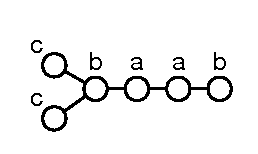
\includegraphics[height=1cm]{graph1}}) with 
vertex labeling  $\pmb{\ell}_{v_1}=\pmb{\ell}_{v_2}=c$,
$\pmb{\ell}_{v_3}=\pmb{\ell}_{v_6}=b$ and $\pmb{\ell}_{v_4}=\pmb{\ell}_{v_5}=a$, and adjacency and degree matrix 
$$
\mathbf{A}:=\begin{bmatrix}
0 & 0 & 1 & 0 & 0 & 0\\
0 & 0 & 1 & 0 & 0 & 0\\
1 & 1 & 0 & 1 & 0 & 0\\
0 & 0 & 1 & 0 & 1 & 0\\
0 & 0 & 0 & 1 & 0 & 1\\
0 & 0 & 0 & 0 & 1 & 0
\end{bmatrix}\text{ and } 
\mathbf{D}:=
\begin{bmatrix}
1 & 0 & 0 & 0 & 0 & 0\\
0 & 1 & 0 & 0 & 0 & 0\\
0 & 0 & 3 & 0 & 0 & 0\\
0 & 0 & 0 & 2 & 0 & 0\\
0 & 0 & 0 & 0 & 2 & 0\\
0 & 0 & 0 & 0 & 0 & 1
\end{bmatrix},
$$
respectively. 
We consider $\mathbf{F}^{(1)}:=\sigma(\tilde{\mathbf{D}}^{-1/2}(\mathbf{A}+\mathbf{I})\tilde{\mathbf{D}}^{-1/2}\mathbf{F}^{(0)}\mathbf{W}^{(0)})$ with  $
\mathbf{F}^{(0)}=
\left[\begin{smallmatrix}
1 & 0 & 0\\
1 & 0 & 0\\
0 & 1 & 0\\
0 & 0 & 1\\
0 & 0 & 1\\
0 & 1 & 0\\
\end{smallmatrix}\right]
$ and choose $\mathbf{W}^{(0)}=\left[\begin{smallmatrix}
1 & 0 & 0\\
0 & 1 & 0\\
0 & 0 & 1
\end{smallmatrix}\right]$. 
We remark that $\pmb{\ell}^{(0)}:=\pmb{\ell}\equiv \mathbf{F}^{(0)}$.
It can be verified that
$$
\mathbf{F}^{(1)}=\sigma\left(\begin{bmatrix}
\frac{1}{2} & \frac{1}{2\sqrt{2}}& 0\\
\frac{1}{2} & \frac{1}{2\sqrt{2}}& 0\\
\frac{1}{2\sqrt{2}} & \frac{1}{4}& \frac{1}{
2\sqrt{3}}\\
0 & \frac{1}{2\sqrt{3}}& \frac{2}{
3}\\
0 & \frac{1}{\sqrt{6}}& \frac{2}{
3}\\
0 & \frac{1}{2}& \frac{1}{
\sqrt{6}}
\end{bmatrix}\right).
$$
Suppose that $\sigma$ is the ReLU activation function. Then, we observe that
$\mathbf{F}^{(1)}_{v_4\bullet}\neq \mathbf{F}^{(1)}_{v_5\bullet}$. 
We note, however, that $\pmb{\ell}^{(1)}_{v_4}=(a,\{a,b\})=\pmb{\ell}^{(1)}_{v_5}$.
Hence, $\pmb{\ell}^{(1)}\not\sqsubseteq \mathbf{F}^{(1)}$ and this architecture is not bounded by WL.
\openprob{Is there a simple example for the one below?}
\qed
% It can, however, be verified that $\pmb{\ell}^{(2)}\sqsubseteq \mathbf{F}^{(1)}$.
% \todo{The latter inclusion needs to be verified}\qed
\end{example}
We will next provide an upper bound for  GNN architectures of the form~(\ref{eq:architecture}) by revising the labeling used in the graph.


\subsection{A general bound}\label{subsec:generalupb}
As we have seen above, for a fair comparison with GNNs of the form~(\ref{eq:architecture}), the WL process needs to have access to the information in the $\mathbf{L}$ and $\mathbf{R}$ matrices. To this aim we extend the set $\Sigma$ of labels.
Let  $(G,\pmb{\ell})$ be a labeled graph and assume that $\pmb{\ell}:V\to \Sigma$. Given $\mathbf{L}$, $\mathbf{R}$  we define $L:=\{ \mathbf{L}_{vv} \mid v\in V\}$ and
$R:=\{ \mathbf{R}_{vv} \mid v\in V\}$.
We define the set $\hat \Sigma$ of \textit{extended labels} as $\hat \Sigma:=\Sigma \cup \Sigma\times L\times R$. Given $(G,\pmb{\ell})$, we consider labeled graph $(G,\hat{\pmb{\ell}})$ with labeling
$$
\hat{\pmb{\ell}}_v:=\langle \pmb{\ell}_v, \mathbf{L}_{vv},\mathbf{R}_{vv}\rangle,
$$
for $v\in V$.
We can now bound the expressive power of  GNN architecture of the form~(\ref{eq:architecture}) by WL \textit{provided that we use the extended labels}. As before, we denote by 
$\hat{\pmb{\ell}}{}^{(t)}$ the labeling obtain after $t$ steps of the WL algorithm on $(G,\hat{\pmb{\ell}})$, starting from $\hat{\pmb{\ell}}{}^{(0)}:=\hat{\pmb{\ell}}$.

\begin{theorem}\label{thm:generalbound}
Let $(G,\pmb{\ell})$ be a labeled graph and assume that $\pmb{\ell}\sqsubseteq\mathbf{F}^{(0)}$.
Then, GNN architectures of the form~(\ref{eq:architecture}) are bounded by WL on $(G,\hat{\pmb{\ell}})$.
\end{theorem}
\begin{proof}
We show the upper bound by WL by induction on the number of iterations. For $t=0$, we have, by assumption, that 
$\pmb{\ell}\sqsubseteq \mathbf{F}^{(0)}$. Clearly,
$\hat{\pmb{\ell}}{}^{(0)}\sqsubseteq \pmb{\ell}$ and hence also 
$\hat{\pmb{\ell}}{}^{(0)}\sqsubseteq\mathbf{F}^{(0)}$. We next assume that the induction hypothesis holds for $t\geq 0$ and consider $t+1$. We need to show that 
$\hat{\pmb{\ell}}{}^{(t+1)}_v=\hat{\pmb{\ell}}{}^{(t+1)}_w$ implies that $\mathbf{F}^{(t+1)}_{v\bullet}=\mathbf{F}^{(t+1)}_{w\bullet}$. By definition,
$\hat{\pmb{\ell}}{}^{(t+1)}_v=\hat{\pmb{\ell}}{}^{(t+1)}_w$ implies
$\hat{\pmb{\ell}}{}^{(t)}_v=\hat{\pmb{\ell}}{}^{(t)}_w$ and 
$$
\ldbl \hat{\pmb{\ell}}{}^{(t)}_u \st u \in N_G(v) \rdbl=
 \ldbl \hat{\pmb{\ell}}{}^{(t)}_u \st u \in N_G(w) \rdbl.$$
 Since $\hat{\pmb{\ell}}{}^{(t)}\sqsubseteq \hat{\pmb{\ell}}{}^{(t-1)}\sqsubseteq \cdots\sqsubseteq \hat{\pmb{\ell}}{}^{(0)}$, this implies that
 $\hat{\pmb{\ell}}{}^{(0)}_v=\hat{\pmb{\ell}}{}^{(0)}_w$ and that there is a bijection $b:N_G(v)\to N_G(w):u\mapsto u'$ such that $\hat{\pmb{\ell}}{}^{(t)}_u=\hat{\pmb{\ell}}{}^{(t)}_{u'}$ and hence also 
 $\hat{\pmb{\ell}}{}^{(0)}_u=\hat{\pmb{\ell}}{}^{(0)}_{u'}$. From the definition of $\hat{\pmb{\ell}}{}^{(0)}$, $\hat{\pmb{\ell}}{}^{(0)}_v=\hat{\pmb{\ell}}{}^{(0)}_w$ implies that
 $\mathbf{L}_{vv}=\mathbf{L}_{ww}$ and
 $\mathbf{R}_{vv}=\mathbf{R}_{ww}$. Similarly, for every $u\in N_G(v)$ and corresponding $u'\in N_G(w)$,
$\hat{\pmb{\ell}}{}^{(0)}_u=\hat{\pmb{\ell}}{}^{(0)}_{u'}$ implies that   $\mathbf{L}_{uu}=\mathbf{L}_{u'u'}$ and $\mathbf{R}_{uu}=\mathbf{R}_{u'u'}$. By the induction hypothesis we also have that
 $\mathbf{F}^{(t)}_{v\bullet}=\mathbf{F}^{(t)}_{w\bullet}$, and for every $u\in N_G(v)$
   and corresponding $u'\in N_G(w)$, $\mathbf{F}^{(t)}_{u\bullet}=\mathbf{F}^{(t)}_{u'\bullet}$. It now suffices to observe that
  \begin{align*}
	  \mathbf{F}^{(t+1)}_{v\bullet}&=\sigma\Biggl(\mathbf{F}^{(t-1)}_{v\bullet}\mathbf{W}_1^{(t-1)}+\mathbf{L}_{vv}\biggl(\Bigl(\sum_{u\in N_G(v)} \mathbf{R}_{uu}\mathbf{F}^{(t)}_{u\bullet}\Bigr)+p\mathbf{R}_{vv}\mathbf{F}^{(t)}_{v\bullet}\biggr)\mathbf{W}^{(t)}+ q\mathbf{J}_{v\bullet}\Biggr)\\
	 & =\sigma\Biggl(\mathbf{F}^{(t-1)}_{w\bullet}\mathbf{W}_1^{(t-1)}+\mathbf{L}_{ww}\biggl(\Bigl(\!\!\sum_{u'\in N_G(w)}\!\! \mathbf{R}_{u'u'}\mathbf{F}^{(t)}_{u'\bullet}\Bigr)+p\mathbf{R}_{ww}\mathbf{F}^{(t)}_{w\bullet}\biggr)\mathbf{W}^{(t)}+ q\mathbf{J}_{w\bullet}\Biggr)\\
	  &=\mathbf{F}^{(t+1)}_{w\bullet},
\end{align*}
as desired.
\end{proof}

\begin{example}\label{ex3}\normalfont
	Continuing with Example~\ref{ex1}, $\hat{\pmb{\ell}}_v:=\langle a,1,1\rangle$ and $\hat{\pmb{\ell}}_w:=\langle a,1,2\rangle$. Hence, $\hat{\pmb{\ell}}{}^{(1)}_v:=(\langle a,1,1\rangle,\{\langle a,1,2\rangle\})$ and $\hat{\pmb{\ell}}{}^{(1)}_w:=(\langle a,1,2\rangle,\{\langle a,1,1\rangle\})$ and $v$ and $w$ are labeled differently in the first step of WL, starting from $\hat{\pmb{\ell}}{}^{(0)}:=\hat{\pmb{\ell}}$. Clearly,
	$\hat{\pmb{\ell}}{}^{(1)}\sqsubseteq \mathbf{F}^{(1)}$ with $\mathbf{F}^{(1)}=\left[\begin{smallmatrix}\sigma(2)\\\sigma(1)\end{smallmatrix}\right]$.
	Continuing with Example~\ref{ex2}, 
$\hat{\pmb{\ell}}_{v_1}=\hat{\pmb{\ell}}_{v_1}:=\langle c, \frac{1}{\sqrt{2}},\frac{1}{\sqrt{2}}\rangle$,
 $\hat{\pmb{\ell}}_{v_3}=\langle b, \frac{1}{\sqrt{4}},\frac{1}{\sqrt{4}}\rangle$, $\hat{\pmb{\ell}}_{v_4}=\hat{\pmb{\ell}}_{v_5}=\langle a, \frac{1}{\sqrt{3}},\frac{1}{\sqrt{3}}\rangle$, and $\hat{\pmb{\ell}}_{v_6}=\langle b,\frac{1}{\sqrt{2}},\frac{1}{\sqrt{2}}\rangle$. Hence, whereas $\pmb{\ell}^{(1)}_{v_4}=\pmb{\ell}^{(1)}_{v_5}$ we now have that
$$
\hat{\pmb{\ell}}{}^{(1)}_{v_4}:=(\langle a, \frac{1}{\sqrt{3}},\frac{1}{\sqrt{3}}\rangle,\{
\langle a, \frac{1}{\sqrt{3}},\frac{1}{\sqrt{3}}\rangle,\langle b, \frac{1}{\sqrt{4}},\frac{1}{\sqrt{4}}\rangle\})
\neq
\hat{\pmb{\ell}}{}^{(1)}_{v_5}:=(\langle a, \frac{1}{\sqrt{3}},\frac{1}{\sqrt{3}}\rangle,\{
\langle a, \frac{1}{\sqrt{3}},\frac{1}{\sqrt{3}}\rangle,\langle b, \frac{1}{\sqrt{2}},\frac{1}{\sqrt{2}}\rangle\}).
$$	It can be verified that $\hat{\pmb{\ell}}{}^{(1)}\sqsubseteq \mathbf{F}^{(1)}$.
	\qed
\end{example}

We will complement Theorem~\ref{thm:generalbound}  with the corresponding lower bound in Section~\ref{sec:lowerb}. In fact, we verify the lower bound already for a slightly simpler class of GNNs than those of the form~(\ref{eq:architecture}).
\floris{It seems that we need lower bounds for two classes (see next section.) So this may need to be revised.}
\begin{theorem}\label{thm:lowerb_general}
The class of GNNs of the form 
\begin{equation}
\mathbf{F}^{(t)}:=\sigma\left(\mathbf{L}(\mathbf{A}+p\mathbf{I})\mathbf{R}\mathbf{F}^{(t-1)}\mathbf{W}^{(t-1)} + q\mathbf{J}\right), \label{eq:architecture_lb}
\end{equation}
is WL-strong, where WL now starts from $(G,\hat{\pmb{\ell}})$. Here, $\sigma$ can be either the sign or the ReLU activation function.
\end{theorem}
This class of GNNs differs from GNNs of the form~(\ref{eq:architecture}) by eliminating  the weight matrices $\mathbf{W}_1^{(t)}$.


\subsection{Special cases}\label{subsec:specialcases}
We next observe that in some cases one can still bound  GNNs of the form~(\ref{eq:architecture}) in terms of WL using the given labeling $\pmb{\ell}$ instead of
$\hat{\pmb{\ell}}$ on $G$. 

% A trivial case for which this holds are adjacency GNNs:
% \begin{description}
%  \item[\textit{Adjacency} (A-GNN):]
% % $\mathbf{L}=\mathbf{R}:=\mathbf{I}$, $p=q:=0$. Hence,
% $
% \mathbf{F}^{(t)}:=\sigma\left(\mathbf{A}\mathbf{F}^{(t-1)}\mathbf{W}^{(t)}\right).
% $
% \end{description}
%
% Indeed, if we consider the adjacency architecture then
% $\hat{\pmb{\ell}}_v:=\langle \pmb{\ell}_v,1,1\rangle$ and thus $\hat{\pmb{\ell}}\equiv\pmb{\ell}$. In this case, the architecture will be bounded by 1-WL
% in the usual way, i.e., starting from $\pmb{\ell}^{(0)}:=\pmb{\ell}$. This holds more generally.
For example, consider GNNs of the form~\ref{eq:groheGNNwithJ}. Here, we have that $\mathbf{L}=\mathbf{R}=\mathbf{I}$. As consequence, for any labeled graph $(G,\pmb{\ell})$
we have that  $\hat{\pmb{\ell}}_v:=\langle \pmb{\ell}_v,1,1\rangle$ and thus $\hat{\pmb{\ell}}\equiv\pmb{\ell}$. In this case, the GNN will be bounded by 1-WL in the usual way, i.e., starting from $\pmb{\ell}^{(0)}:=\pmb{\ell}$. 

\begin{corollary}\label{cor:adjacency}
GNNs of the form~(\ref{eq:architecture}) for which 
$\pmb{\ell}\sqsubseteq\hat{\pmb{\ell}}$ holds, for any labeled graph $(G,\pmb{\ell})$, are bounded by WL, starting from $\pmb{\ell}^{(0)}:=\pmb{\ell}$. 
% In particular, the adjacency architecture is bounded by 1-WL.
\end{corollary}
\begin{proof}
For any labeled graph $(G,\pmb{\ell})$ we always have that $\hat{\pmb{\ell}}\sqsubseteq \pmb{\ell}$. Hence, the assumption $\pmb{\ell}\sqsubseteq\hat{\pmb{\ell}}$ implies that $\pmb{\ell}\equiv\hat{\pmb{\ell}}$. As a consequence, $\pmb{\ell}^{(t)}\equiv \hat{\pmb{\ell}}{}^{(t)}$ for all $t\geq 0$. Theorem~\ref{thm:generalbound} then implies $\hat{\pmb{\ell}}{}^{(t)}\sqsubseteq \mathbf{F}^{(t)}$, and hence also $\pmb{\ell}^{(t)}\sqsubseteq\mathbf{F}^{(t)}$.
\end{proof}
Intuitively, if $\pmb{\ell}\sqsubseteq\hat{\pmb{\ell}}$ holds for any labeled graph $(G,\pmb{\ell})$, then this implies that the matrices $\mathbf{L}$ and $\mathbf{R}$ must
be constant. Indeed, just consider the uniform labeling $\pmb{\ell}_v:=a$ for all $v\in V$. Then,
$\pmb{\ell}\equiv\hat{\pmb{\ell}}$ if and only if $\mathbf{L}_{vv}=\mathbf{L}_{ww}$
and $\mathbf{R}_{vv}=\mathbf{R}_{ww}$ for all vertices.
This is clearly the case for GNNs of the form~(\ref{eq:groheGNNwithJ}).
Another way of verifying Corollary~\ref{cor:adjacency} is that when $\mathbf{L}$ and $\mathbf{R}$ are constant, then GNNs of the form
~(\ref{eq:architecture}) can be seen as GNN of the form~\ref{lab:generalGNN}, and Proposition~\ref{prop:upperboundgeneral} applies.

In view of Corollary~\ref{cor:adjacency}, we remark that Theorem~\ref{thm:lowerb_general} implies that when $\mathbf{L}$ and $\mathbf{R}$ are constant matrices, the corresponding class of GNNs is WL-strong, starting from $(G,\pmb{\ell})$. This holds in particular
for the class of GNNs of the form~\ref{eq:groheGNNwithJ}. Hence, we recover the result from~\cite{grohewl} stating that GNNs of the form~\ref{eq:groheGNNwithJ} are WL-strong. Furthermore, as anticipated, the lower bound also holds for the ReLU function. We defer the details of the lower bounds to Section~\ref{sec:lowerb}.

As a second example, consider a NA-GNN+. For those GNNs, we have that $\mathbf{L}_{vv}=\frac{1}{\sqrt{1+d_v}}$
and $\mathbf{R}_{vv}=\frac{1}{\sqrt{1+d_v}}$. This implies that
for any labeled graph $(G,\pmb{\ell})$ we have that $\pmb{\ell}^{(1)}\sqsubseteq\hat{\pmb{\ell}}$
holds. Indeed, if $\pmb{\ell}^{(1)}_v=\pmb{\ell}^{(1)}_w$ then $\pmb{\ell}_v=\pmb{\ell}_w$ and for every $u\in N_G(v)$ and corresponding $u'\in N_G(w)$,
$\pmb{\ell}_u=\pmb{\ell}_{u'}$. In particular, $d_{v}=d_w$ and thus  $\pmb{\ell}^{(1)}\sqsubseteq\hat{\pmb{\ell}}$. More generally, if $\pmb{\ell}^{(1)}\sqsubseteq\hat{\pmb{\ell}}$ holds for any labeled graph $(G,\pmb{\ell})$,
then the entries of $\mathbf{L}$ and $\mathbf{R}$ must be functionally determined by the
degrees of the vertices. To see this, it suffices to consider again the uniform labeling
$\pmb{\ell}_v:=a$ for all $v\in V$. Then, $\pmb{\ell}^{(1)}\sqsubseteq\hat{\pmb{\ell}}$ implies that
for any two vertices $v$ and $w$, 
$$(a,\underbrace{\ldbl a, a,\ldots, a\rdbl}_{|N_G(v)|=d_v})=
(a,\underbrace{\ldbl a, a,\ldots, a\rdbl}_{|N_G(w)|=d_w}),$$
or in other words, $d_v=d_w$. So, when  $d_v=d_w$ we have $\hat{\pmb{\ell}}_v=\hat{\pmb{\ell}}_w$, or $d_v=d_w$ implies $\mathbf{L}_{vv}=\mathbf{L}_{ww}$ and $\mathbf{R}_{vv}=\mathbf{R}_{ww}$.

\begin{corollary}\label{cor:augmented2}
GNNs of the form~(\ref{eq:architecture}) for which 
$\pmb{\ell}^{(1)}\sqsubseteq\hat{\pmb{\ell}}$ holds, for any labeled graph $(G,\pmb{\ell})$, are bounded by WL, starting from $\pmb{\ell}^{(1)}$. 
\end{corollary}
\begin{proof}
If 	$\pmb{\ell}^{(1)}\sqsubseteq\hat{\pmb{\ell}}$ holds, then also 
$\pmb{\ell}^{(t+1)}\sqsubseteq\hat{\pmb{\ell}}{}^{(t)}$ holds for any $t\geq 0$. Hence,
$\pmb{\ell}^{(t+1)}\sqsubseteq \mathbf{F}^{(t)}$ 
% or $\pmb{\ell}^{(1)}\sqsubseteq\mathbf{F}^{(t-1)}$ by
by Theorem~\ref{thm:generalbound}.
\end{proof}

This upper bound holds for all special GNNs listed at the end of the previous section. Indeed,
Indeed, $\hat{\pmb{\ell}}_v:=\langle \pmb{\ell}_v,1,1\rangle$ for GNNs of the form ~(\ref{eq:groheGNNwithJ}),
$\hat{\pmb{\ell}}_v:=\langle \pmb{\ell}_v,1/d_{v},1\rangle$ for RW-GNNS,
$\hat{\pmb{\ell}}_v:=\langle \pmb{\ell}_v,1/\sqrt{d_{v}},1/\sqrt{d_{v}}\rangle$ for NA-GNNs,1-GCN's and 1-GCNs's, 
$\hat{\pmb{\ell}}_v:=\langle \pmb{\ell}_v,1/\sqrt{1+d_{v}},1\rangle$ for RW-GNN+
$\hat{\pmb{\ell}}_v:=\langle \pmb{\ell}_v,1/\sqrt{1+d_{v}},1/\sqrt{1+d_{v}}\rangle$ for NA-GNN+, as we have seen already above, and 
$\hat{\pmb{\ell}}_v:=\langle \pmb{\ell}_v,1/\sqrt{r+(1-r)d_{v}},1/\sqrt{r+(1-r)d_{v}}\rangle$ 
for NA-GNN++.

We note than when a GNN is bounded by WL, starting from $\pmb{\ell}^{(k)}$, it is also bounded by WL, starting from $\pmb{\ell}^{(k')}$ for all $k'\geq k$. The converse is not necessarily true, as is illustrated by the following example for NA-GNN+'s.
\begin{example}\label{ex4}\normalfont
Going back to  Example~\ref{ex2}, we know from Corollary~\ref{cor:augmented2} that NA-GNN+'s are bounded WL, starting from $\pmb{\ell}^{(1)}$. It can indeed be verified that in Example~\ref{ex2}, $\pmb{\ell}^{(2)}\sqsubseteq \mathbf{F}^{(1)}$. We have seen, however, that $\pmb{\ell}^{(1)}\not\sqsubseteq \mathbf{F}^{(1)}$. Hence, NA-GNN+'s are not necessarily bounded by WL, starting from $\pmb{\ell}^{(0)}$.\qed
\end{example}
It can also be verified that the previous example works for 1-GCNs's (and thus also for 1-GCN's) and NA-GNN's (and thus also NA-GNN++'s).
\begin{example}\normalfont
	Using the same setting as in Example~\ref{ex2}, it can be verified that 
	$$\mathbf{F}^{(1)}=\sigma\left(\begin{bmatrix}
	1 & 1/6 & 0\\
	1 & 1/6 & 0\\
	1/3 & 1 & 1/6\\
	0 & 1/6 & 5/4\\
	0 & 1/2 & 5/4\\
    0 & 1 & 1/2	\end{bmatrix}\right) \text{ and }
 \mathbf{F}^{(1)}=\sigma\left(\begin{bmatrix}
	0 & 1/6 & 0\\
	0 & 1/6 & 0\\
	1/3 & 0 & 1/6\\
	0 & 1/6 & 1/4\\
	0 & 1/2 & 1/4\\
    0 & 0 & 1/2	\end{bmatrix}\right), $$
	for 1-GCNs and for NA-GNNs, respectively. In both case, we see that $\pmb{\ell}^{(1)}\not\sqsubseteq \mathbf{F}^{(1)}$. Hence, these architectures are not necessarily bounded by WL, starting from $\pmb{\ell}$.\qed
\end{example}


We will complement Corollary~\ref{cor:augmented2} by the following lower bound in Section~\ref{sec:lowerb}.
\floris{Again, we need two such results, in order to capture all our GNN architectures. See next section.}

\begin{theorem}
GNNs of the form~(\ref{eq:architecture}) for which 
$\pmb{\ell}^{(1)}\sqsubseteq\hat{\pmb{\ell}}$ holds, for any labeled graph $(G,\pmb{\ell})$, are WL-strong, starting from $\pmb{\ell}^{(1)}$. 
\end{theorem}
In particular, we show this lower bound holds already for GNNs of the form~(\ref{eq:architecture_lb})
for which $\pmb{\ell}^{(1)}\sqsubseteq\hat{\pmb{\ell}}$ holds, for any labeled graph $(G,\pmb{\ell})$.



% Corollary~\ref{cor:augmented} applies for $k=1$ for the random walk, normalized adjacency, augmented random walk and augmented adjacency architectures. Indeed, for these architectures,
% $\hat{\pmb{\ell}}_v:=\langle \pmb{\ell}_v,1/d_{v},1\rangle$,
% $\hat{\pmb{\ell}}_v:=\langle \pmb{\ell}_v,1/\sqrt{d_{v}},1/\sqrt{d_{v}}\rangle$,
% $\hat{\pmb{\ell}}_v:=\langle \pmb{\ell}_v,1/\sqrt{1+d_{v}},1\rangle$, and
% $\hat{\pmb{\ell}}_v:=\langle \pmb{\ell}_v,1/\sqrt{(1+d_{v})},1/\sqrt{(1+d_{v}})\rangle$, respectively. For none of these architecture the inclusion $\pmb{\ell}\sqsubseteq \hat{\pmb{\ell}}$ necessarily holds. We note, however, that when $\pmb{\ell}^{(1)}_v=\pmb{\ell}^{(1)}_w$ then $\pmb{\ell}_v=\pmb{\ell}_w$ and for every $u\in N_G(v)$ and corresponding $u'\in N_G(w)$,
% $\pmb{\ell}_u=\pmb{\ell}_{u'}$. In particular, $d_{v}=d_w$. Hence, $\pmb{\ell}^{(1)}\sqsubseteq\hat{\pmb{\ell}}$. As a consequence,  Corollary~\ref{cor:augmented} implies:
% \begin{corollary}\label{cor:augmented2}
% The random walk, normalized adjacency, augmented random walk and augmented adjacency architectures are  bounded by 1-WL, starting from $\pmb{\ell}^{1}$.
% \end{corollary}


A careful look at the  proof of Theorem~\ref{thm:generalbound} reveals that
the roles of $\mathbf{L}$ and $\mathbf{R}$ in the GNN architectures~(\ref{eq:architecture})
are different. Indeed, if we wish to compute the feature vector $\mathbf{F}^{(t+1)}_{v\bullet}$ of a vertex $v$, then only $\mathbf{L}_{vv}$
is required from $\mathbf{L}$. By contrast, we need  $\mathbf{R}_{vv}$ and $\mathbf{R}_{uu}$ for every $u\in N_G(v)$ from $\mathbf{R}$. As it turns out,
even when $\hat{\pmb{\ell}}\not\equiv \pmb{\ell}$, it is sometimes the case that the architecture is still bounded by WL, starting from $\pmb{\ell}$. 

For example, if we take any of the GNNs for which $\mathbf{L}$ is functionally determined by
the degrees of vertices and for which $\mathbf{R}=\mathbf{I}$, then for any labeled graph $(G,\pmb{\ell})$ we have that $\pmb{\ell}^{(1)}\sqsubseteq \hat{\pmb{\ell}}$ holds, as before. In addition, however, we have that $\pmb{\ell}_v=\pmb{\ell}_w\Rightarrow \mathbf{R}_{vv}=\mathbf{R}_{ww}$. It is easy to see that this condition  corresponds to 
$\mathbf{L}$ being functionally determined by degree information, and $\mathbf{R}$ being a constant matrix. We remark that these conditions are satisfied for RW-GNNs and RW-GNN+'s
and GNNs of the form~\ref{eq:groheGNNwithJ}. 

\begin{corollary}\label{cor:weak}
	GNNs of the form~(\ref{eq:architecture}) for which 
	$\pmb{\ell}^{(1)}\sqsubseteq\hat{\pmb{\ell}}$  and
	$\pmb{\ell}^{(0)}_v=\pmb{\ell}^{(0)}_w\Rightarrow \mathbf{R}_{vv}=\mathbf{R}_{ww}$ hold,
 for any labeled graph $(G,\pmb{\ell})$, are bounded by WL, starting from $\pmb{\ell}$.
% For any $k'<k$ such that $\pmb{\ell}^{(k)}\sqsubseteq \hat{\pmb{\ell}}$ and
% $\pmb{\ell}^{(k')}_v=\pmb{\ell}^{(k')}_w\Rightarrow \mathbf{R}_{vv}=\mathbf{R}_{ww}$ hold, we have that GNN architectures of the form~(\ref{eq:architecture})  are bounded by 1-WL, starting from $\pmb{\ell}^{(k-1)}$.
\end{corollary}
\begin{proof}
We need to show that $\pmb{\ell}^{(t)}_v=\pmb{\ell}^{(t)}_w$ implies $\mathbf{F}^{(t)}_{v\bullet}=\mathbf{F}^{(t)}_{w\bullet}$ for $t\geq 0$.
We show this by induction on $t$. For $t=0$, we have by assumption that $\pmb{\ell}^{(0)}\sqsubseteq \mathbf{F}^{(0)}$.
 % and since $\pmb{\ell}^{(k-1)}\sqsubseteq\pmb{\ell}^{(0)}$ also $\pmb{\ell}^{(k-1)}\sqsubseteq\mathbf{F}^{(0)}$.
 Consider $t\geq 1$ and assume that $\pmb{\ell}^{(t)}_v=\pmb{\ell}^{(t)}_w$. This implies that $\pmb{\ell}^{(t-1)}_v=\pmb{\ell}^{(t-1)}_w$ and for every $u\in N_G(v)$ and corresponding $u'\in N_G(w)$, $\pmb{\ell}^{(t-1)}_u=\pmb{\ell}^{(t-1)}_{u'}$.
By induction, $\mathbf{F}^{(t-1)}_{v\bullet}=\mathbf{F}^{(t-1)}_{w\bullet}$ and for every $u\in N_G(v)$ and corresponding $u'\in N_G(w)$,  $\mathbf{F}^{(t-1)}_{u\bullet}=\mathbf{F}^{(t-1)}_{u'\bullet}$. 
We observe that $\pmb{\ell}^{(t)}_v=\pmb{\ell}^{(t)}_w$ implies that
$\pmb{\ell}^{(1)}_v=\pmb{\ell}^{(1)}_w$ since $t\geq 1$.
Hence,
% $\pmb{\ell}^{(1)}\sqsubseteq \hat{\pmb{\ell}}$ for $t\geq k$. Hence,
$\mathbf{L}_{vv}=\mathbf{L}_{ww}$ and $\mathbf{R}_{vv}=\mathbf{R}_{ww}$. Furthermore, 
$\pmb{\ell}^{(t-1)}_u=\pmb{\ell}^{(t-1)}_{u'}$ does not necessary implies that 
$\pmb{\ell}^{(1)}_v=\pmb{\ell}^{(1)}_w$ (e.g., when $t=1$). It does, however imply that
$\pmb{\ell}_u=\pmb{\ell}_{u'}$ and hence, by assumption, $\mathbf{R}_{uu}=\mathbf{R}_{u'u'}$. 
Hence, also $\pmb{\ell}^{(t-1)}_u=\pmb{\ell}^{(t-1)}_{u'}\Rightarrow \mathbf{R}_{uu}=\mathbf{R}_{u'u'}$.
Hence,
$\pmb{\ell}^{(t-1)}_u=\pmb{\ell}^{(t-1)}_{u'}$ implies $\mathbf{R}_{uu}=\mathbf{R}_{u'u'}$ for every $u\in N_G(v)$ and corresponding $u'\in N_G(w)$.
This suffices to conclude that 
  \begin{align*}
	  \mathbf{F}^{(t)}_{v\bullet}&=\sigma\Biggl(\mathbf{F}^{(t-1)}_{u\bullet}\mathbf{W}_1^{(t-1)}+\mathbf{L}_{vv}\biggl(\Bigl(\sum_{u\in N_G(v)} \mathbf{R}_{uu}\mathbf{F}^{(t-1)}_{u\bullet}\Bigr)+p\mathbf{R}_{vv}\mathbf{F}^{(t-k)}_{v\bullet}\biggr)\mathbf{W}^{(t-1)}+ q\mathbf{J}_{v\bullet}\Biggr)\\
	 & =\sigma\Biggl(\mathbf{F}^{(t-1)}_{v\bullet}\mathbf{W}_1^{(t-1)}+\mathbf{L}_{ww}\biggl(\Bigl(\!\!\sum_{u'\in N_G(w)}\!\! \mathbf{R}_{u'u'}\mathbf{F}^{(t-1)}_{u'\bullet}\Bigr)+p\mathbf{R}_{ww}\mathbf{F}^{(t-1)}_{w\bullet}\biggr)\mathbf{W}^{(t-1)}+ q\mathbf{J}_{w\bullet}\Biggr)\\
	  &=\mathbf{F}^{(t)}_{w\bullet},
\end{align*}
as desired.
\end{proof}

We will  show in the next section that GNNs of the form~(\ref{eq:architecture}) for which 
$\pmb{\ell}^{(1)}\sqsubseteq\hat{\pmb{\ell}}$  and 
	$\pmb{\ell}^{(0)}_v=\pmb{\ell}^{(0)}_w\Rightarrow \mathbf{R}_{vv}=\mathbf{R}_{ww}$ hold,
 for any labeled graph $(G,\pmb{\ell})$, are also WL-strong,  starting from $\pmb{\ell}$.
 
 

%
%
%
% %
% % As we will see shortly, this holds for the random walk and augmented random walk architectures.
% % % We start by identifying conditions on
% % $\hat{\pmb{\ell}}$ that result in the architecture to be only $k-1$ steps ahead of $1$-WL, rather than $k$-steps ahead as reported in Corollary~\ref{cor:augmented}.
%
% \begin{corollary}\label{cor:weak}
% For any $k'<k$ such that $\pmb{\ell}^{(k)}\sqsubseteq \hat{\pmb{\ell}}$ and
% $\pmb{\ell}^{(k')}_v=\pmb{\ell}^{(k')}_w\Rightarrow \mathbf{R}_{vv}=\mathbf{R}_{ww}$ hold, we have that GNN architectures of the form~(\ref{eq:architecture})  are bounded by 1-WL, starting from $\pmb{\ell}^{(k-1)}$.
% \end{corollary}
% We remark that the assumptions on  $\pmb{\ell}$ and $\hat{\pmb{\ell}}$ are satisfied for the
% random walk and augmented random walk architectures. Indeed, for these architectures,
% $\hat{\pmb{\ell}}_v:=\langle \pmb{\ell}_v,1/d_{v},1\rangle$ and
% $\hat{\pmb{\ell}}_v:=\langle \pmb{\ell}_v,1/\sqrt{1+d_{v}},1\rangle$, respectively. We have seen before that
% $\pmb{\ell}^{(1)}\sqsubseteq \hat{\pmb{\ell}}$. Moreover, $\pmb{\ell}^{(0)}_v=\pmb{\ell}^{(0)}_w$ implies
% $\mathbf{R}_{vv}=1=\mathbf{R}_{ww}$. Hence, Corollary~\ref{cor:weak}, for $k=1$ and $k'=0$, implies:
%
% \begin{corollary}\label{cor:augrw1wl}
% The random walk and augmented random walk architectures are bounded by 1-WL, starting from $\pmb{\ell}^{(0)}$.
% \end{corollary}
%
% It remains to show Corollary~\ref{cor:weak}. The proof is minor modification of the proof of Theorem~\ref{thm:generalbound}.


We can now use this lemma and continue in the same way as in~\cite{grohewl}:
\begin{theorem}\label{thm:relu}
Let $G$ be an unlabeled graph without isolated vertices and represented by adjacency matrix $\mathbf{A}$. Then there exist weight matrices $\mathbf{W}^{(t)}$
and constants $m^{(t)}$ such that the vertex labelling induced by 
\begin{equation}
  \mathbf{F}^{(t+1)} = \text{\normalfont ReLU}\left(
    \mathbf{A}\mathbf{F}^{(t)}\mathbf{W}^{(t)} - m^{(t)}\mathbf{J}  \right)
\end{equation}
is equivalent to the vertex labelling $\ell^{(t+1)}$ induced by 1-WL.
\end{theorem}
\todo{G: so then here we are missing a self-contained proof of the claim,
following Grohe, right?}
\todo{F: I was thinking that we could give an overview of the proof at the start of the appendix, highlighting
what is needed to make the argument go through (row-independences, preservation of equivalence of 
1-WL at each iteration, Lemma 9, ...). Alternatively, we write down the proofs for each case over and over again.}
In other words, GNNs of the form   $\mathbf{F}^{(t+1)} = \sigma\left(
    \mathbf{A}\mathbf{F}^{(t)}\mathbf{W}^{(t)} - m^{(t)}\mathbf{J}  \right)$
are as powerful as 1-WL, when $\sigma$ is either sign or ReLU, on unlabeled graphs.

\paragraph{Kipf+bias}
We next consider GNNs based on~\cite{kipf-loose}. Let $\mathbf{D}$ be the \emph{degree matrix} of $G$, that is $\mathbf{D}$
is the diagonal matrix such that
$    \mathbf{D}_{ii} = |N_G(i)|$. We will now consider GNNs of the form
\begin{equation}\label{GNN:Kipf}
    \mathbf{F}^{(t+1)} = \sigma\left(
        \mathbf{D}^{-1/2}\mathbf{A}\mathbf{D}^{-1/2}
        \mathbf{F}^{(t)}\mathbf{W}^{(t)} + m^{(t)}\mathbf{J}
    \right),
\end{equation}
where $\mathbf{D}^{-1/2}$
is the diagonal matrix with
$\mathbf{D}^{-1/2}_{ii} =
\frac{1}{\sqrt{\mathbf{D}_{ii}}}$ and $m^{(t)}$ is a bias factor\footnote{No bias was consider in~\cite{kipf-loose}. Kipf uses $\mathbf{A}+\mathbf{I}$ instead of $\mathbf{A}$.}.
We show that GNNs of this form are also as powerful as 1-WL. This connection was mentioned in~\cite{kipf-loose} but not made precise. We do not know whether it holds when no bias is allowed.

To show that GNNs of the form~(\ref{GNN:Kipf}) are as powerful as 1-WL,
we first show that GNNs
of the form 
\begin{equation}\label{eq:halfkipf}
    \mathbf{F}^{(t+1)} = \sigma\left(
        \mathbf{A}\mathbf{D}^{-1/2}
        \mathbf{F}^{(t)}\mathbf{W}^{(t)} + m^{(t)}\mathbf{J}
    \right),
\end{equation}
are as powerful as 1-WL.  To see why this holds,   we write~(\ref{eq:halfkipf}) as:
\begin{align*}
\mathbf{G}^{(t)} &= \mathbf{D}^{-1/2}\mathbf{F}^{(t)}\\
\mathbf{F}^{(t+1)} &= \sigma\left(
    \mathbf{A}\mathbf{G}^{(t)}\mathbf{W}^{(t)} - m^{(t)}\mathbf{J}  \right),
\end{align*}    
and argue that the construction of weight matrices as given in~\cite{grohewl} for the sign function and Theorem~\ref{thm:relu} for the ReLU function can be used to simulate 1-WL.

We first observe that $\mathbf{G}^{(0)}=\mathbf{D}^{-1/2}\mathbf{F}^{(0)}=\mathbf{D}^{-1/2}\mathbf{J}$. \todo{G: here we seem to be assuming a specific encoding of the initial labelling into the feature vectors, right?}
\todo{Floris: this is the unlabeled case, so the initial feature vector will be all ones.}
Hence, we see that 
the vertex labelling induced by $\mathbf{G}^{(0)}$ corresponds to $\ell^{(1)}$, i.e., the vertex labelling of 1-WL after one iteration. A crucial property underlying the construction of the weight matrices $\mathbf{W}^{(t)}$ to simulate 1-WL is that the feature vectors are row-independent modulo equality. That is, the \textit{set} of all row vectors  are linearly independent. 
Clearly, $\mathbf{G}^{(0)}$ satisfies this property. Furthermore, when $\mathbf{G}^{(t)}$ is row-independent modulo equality, then the 
construction of the weight matrices and bias, ensure that $\mathbf{F}^{(t+1)}$ is also row-independent modulo equality. We next argue that
also $\mathbf{G}^{(t+1)}$ has this property. Indeed, $\mathbf{G}^{(t+1)}_{i\bullet}=\frac{1}{\sqrt{\mathbf{D}_{ii}}} \mathbf{F}^{(t+1)}_{i\bullet}$ and thus $\mathbf{G}^{(t+1)}$ consists of scalar multiples of $\mathbf{F}^{(t+1)}$.

We next show correctness, i.e., the vertex labelling induced by $\mathbf{F}^{(t+1)}$  is equivalent to the vertex labelling $\ell^{(t+1)}$ induced by 1-WL.
For the base, $t=0$, since the vertex labelling induced by  $\mathbf{G}^{(0)}$ corresponds to $\ell^{(1)}$, then $\mathbf{F}^{(1)}$ corresponds to $\ell^{(2)}$. For $t>0$, assume that the vertex labelling induced by $\mathbf{F}^{(t)}$ is equivalent to $\ell^{(t+1)}$. It suffices to show that 
$\mathbf{G}^{(t)}$ is also equivalent to $\ell^{(t+1)}$. Then, the construction of weight matrices given in~\cite{grohewl} (for sign) and Theorem~\ref{thm:relu} (for ReLU) ensure that the vertex labelling induced by $\mathbf{F}^{(t+1)}$ is equivalent to $\ell^{(t+2)}$.

So, assume that  $\mathbf{F}^{(t)}$ is equivalent to $\ell^{(t+1)}$. We observe that vertices with different degrees will be labelled differently by 1-WL in each iterations. Hence,  if $\mathbf{F}^{(t)}_{i\bullet}=\mathbf{F}^{(t)}_{j\bullet}$ then $\mathbf{D}_{ii}=\mathbf{D}_{jj}$ and hence, $\mathbf{G}^{(t)}_{i\bullet}=\mathbf{G}^{(t)}_{j\bullet}$. Furthermore, assume that $\mathbf{G}^{(t)}_{i\bullet}= \mathbf{G}^{(t)}_{j\bullet}$ but $\mathbf{F}^{(t)}_{i\bullet}\neq \mathbf{F}^{(t)}_{j\bullet}$. Then this implies that  $\mathbf{F}^{(t)}_{i\bullet}$ and $\mathbf{F}^{(t)}_{j\bullet}$ are scalar multiples of each other. This contradicts that  $\mathbf{F}^{(t)}$ is row-independent modulo equality. As a consequence, the vertex labellings induced by  $\mathbf{F}^{(t)}$ and $\mathbf{G}^{(t)}$ are equivalent, and hence equivalent to $\ell^{(t+1)}$.  It remains to verify that $\mathbf{F}^{(t)}_{i\bullet}=\mathbf{F}^{(t)}_{j\bullet}$ implies $\mathbf{D}_{ii}=\mathbf{D}_{jj}$, or equivalently, that 
    $\ell^{(t+1)}_i=\ell^{(t+1)}_j$ implies $\mathbf{D}_{ii}=\mathbf{D}_{jj}$. This clearly holds because the degree information is already encoded in $\ell^{(1)}$ in 1-WL and hence also in vertex labelling in further iterations of 1-WL.

\begin{proposition}
Let $G$ be an unlabeled graph without isolated vertices and represented by adjacency matrix $\mathbf{A}$. Then there exist weight matrices $\mathbf{W}^{(t)}$
and constants $m^{(t)}$ such that the  vertex labelling induced by 
\begin{equation}
  \mathbf{F}^{(t+1)} = \sigma\left(
    \mathbf{A}\mathbf{D}^{-1/2}\mathbf{F}^{(t)}\mathbf{W}^{(t)} - m^{(t)}\mathbf{J}  \right)
\end{equation}
is equivalent to the vertex labelling $\ell^{(t+2)}$ induced by 1-WL.
\end{proposition}

We next consider GNNs of the form 
\begin{equation}
    \mathbf{F}^{(t+1)} = \sigma\left(
        \mathbf{D}^{-1/2}\mathbf{A}\mathbf{D}^{-1/2}
        \mathbf{F}^{(t)}\mathbf{W}^{(t)} + m^{(t)}\mathbf{J}
    \right),
\end{equation}

We show that Lemma 9 from~\cite{grohewl} (for sign) and Lemma~\ref{lem:relulemma9} (for ReLU) can be extended to
this case. Without the initial factor  $\mathbf{D}^{-1/2}$,  the input matrix $\mathbf{B}$ in these lemmas consist of $\widetilde{\mathbf{A}\mathbf{D}^{-1/2} \mathbf{F}^{(t)}}$, the matrix obtained from $\mathbf{A}\mathbf{D}^{-1/2} \mathbf{F}^{(t)}$ by only considering its  unique rows. Let us denote  $\mathbf{A}\mathbf{D}^{-1/2} \mathbf{F}^{(t)}$ by $\mathbf{Z}^{(t)}$. 
We have seen above that $(\mathbf{Z}^{(t)})_{i\bullet}=(\mathbf{Z}^{(t)})_{j\bullet}$ implies that $D_{ii}=D_{jj}$. 
Furthermore, the unique rows in $\mathbf{Z}$ are linearly independent. So, when  $(\mathbf{Z}^{(t)})_{i\bullet}\neq (\mathbf{Z}^{(t)})_{j\bullet}$ then there are no scalars $c$ and $d$ such that $c(\mathbf{Z}^{(t)})_{i\bullet}= d(\mathbf{Z}^{(t)})_{j\bullet}$.
This implies that the only effect that the initial factor $\mathbf{D}^{-1/2}$ has rescales rows whilst preserving row-equality. 
In other words, $\widetilde{\mathbf{D}^{-1/2}\mathbf{A}\mathbf{D}^{-1/2} \mathbf{F}^{(t)}}$ will consist of the rows in 
$\widetilde{\mathbf{A}\mathbf{D}^{-1/2} \mathbf{F}^{(t)}}$ scaled with the appropriate $1/{\sqrt{D_{ii}}}$. And, the same rows in 
$\mathbf{A}\mathbf{D}^{-1/2} \mathbf{F}^{(t)}$ will be rescaled with same factor. So, we end up with  $\widetilde{\mathbf{D}^{-1/2}\mathbf{A}\mathbf{D}^{-1/2} \mathbf{F}^{(t)}}$ being row-independent modulo equality.... again show it provides a correct vertex labelling??

\todo{It feels that these arguments are too repetitive. What we should try to have is some key lemmas that when valid, guarantee correctness.}
    

\paragraph{Including self-loops}
In Kipf, $\mathbf{A}+\mathbf{I}$ is used instead of $\mathbf{A}$. We can either just argue that this is just 1-WL but now for graphs with self-loops. Alternatively, papers make a fuzz about this ``normalisation trick''. Can we say something more about this?


\subsection{Labeled graphs}


\newpage




\subsection{Old stuff}


%
%
%
%It is now easy to see that we can define weight matrices such that
%\[
%    \mathbf{F}^{(t+1)} = \textsf{ReLU}\left(\mathbf{AF}^{(t)}\mathbf{W}^{(t)}-m^{(t)}\mathbf{J}\right).
%\]
%is again equivalent to $c_\ell^{(t+1)}$.  We show that we modify $\mathbf{F}^{(t)}$ and $\mathbf{W}^{(t)}$
%such that can rewrite the update rule in Kipf form.
%
%Let $\mathbf{d}^{(t)}:=\mathbf{A}^{t}\mathbf{1}^\textsc{t}$. That is, $\mathbf{d}^{(t)}_v$ counts the paths from vertex $v$ of length $t$. We note that for undirected graphs $\mathbf{d}^{(t)}$ holds non-negative entries\footnote{For directed graphs, we may consider $I+A$ instead.}
%We now use a similar construction of $\mathbf{W'}^{(t)}$ in the proof of Theorem~\ref{thm:simpler-grohe}, i.e.,
%\[
%\mathbf{W'}^{(t)}=\begin{pmatrix}
%\mathbf{W}^{(t)} & \mathbf{0}_{d\times 1}\\
%\left(-\frac{m^{(t)}}{d_1^{(t+1)}},\ldots,-\frac{m^{(t)}}{d_n^{(t+1)}}\right) & 1
%\end{pmatrix}.
%\]
%and we replace $\mathbf{F}$ by $\mathbf{F'}=[\mathbf{F},\mathbf{1}]$. Then,
%\begin{align}
%    \mathbf{F'}^{(t+1)} 
%        &=\textsf{ReLU}(\mathbf{A}\mathbf{F'}\mathbf{W'}^{(t)}) \nonumber \\
%        &=[\textsf{ReLU}(\mathbf{A}\mathbf{F}^{(t)}\mathbf{W}^{(t)}-m^{(t)}\mathbf{J}),\textsf{ReLU}(\mathbf{d}^{(t+1)})]. \nonumber \\
%        &=[\mathbf{F}^{(t+1)}, \mathbf{d}^{(t+1)}] \label{eq:Fc}
%\end{align}
%It now suffices to show that $\mathbf{F'}^{(t)}$ is equivalent to $c_\ell^{(t)}$. Since $\mathbf{F}^{(t)} \equiv c_\ell^{(t)}$ and by~\eqref{eq:Fc} $\mathbf{F'}^{(t+1)} \sqsubseteq \mathbf{F}^{(t+1)}$ it suffices to prove that $c_\ell^{(t)} \sqsubseteq \mathbf{F'}^{(t)}$.
%This boils down to the following lemma.
%
%\begin{lemma}\label{lem:deg-in-WL}
%    Let $(G,c)$ be a labeled graph.
%    Then for all $t \geq 0$ we have that 
%    $c_\ell^{(t)} \sqsubseteq \mathbf{d}^{(t)}$. \filip{I think it's a bit ugly that $c$ is a function and $d$ is a vector but I find this statement better. Maybe we should define $c$ in bold (as a vector)?}
%%     \[
%%         c^{(t)}(u) = c^{(t)}(v) \implies d^{(t)}_u = d^{(t)}_v.
%%     \]
%\end{lemma}
%\begin{proof}
%Since $c_\ell^{(0)}$ assigns every vertex the same label, and $\mathbf{d}^{(0)}=\mathbf{1}^t$, our hypothesis holds for the base case.
%%Filip: I started modifying here
%For the induction step suppose that $c_\ell^{(t-1)}(v)=c_\ell^{(t-1)}(w)$ implies $\mathbf{d}^{(t-1)}_v=\mathbf{d}^{(t-1)}_w$.
%Given a label $c$ we will use the notation $\mathbf{d}^{(t-1)}_c$, which is equal to $\mathbf{d}^{(t-1)}_v$ for any $v$ such that $c_\ell^{(t-1)} = c$. By the induction assumption this definition does not depend on the choice of $v$.
%
%Take two vertices $v$ and $w$ such that $c_\ell^{(t)}(v)=c_\ell^{(t)}(w)$. By definition of the 1-WL algorithm 
%$$
%|N_G(v)\cap (c_\ell^{(t-1)})^{-1}(c)|=|N_G(w)\cap (c_\ell^{(t-1)})^{-1}(c)|
%$$
%for any label $c$ in ${\cal C}^{(t-1)}$ (i.e., the image of $c_\ell^{(t-1)}(V)$). Then
%\begin{align*}
%\mathbf{d}^{(t)}_v&=\sum_{x\in N_G(v)} \mathbf{d}^{(t-1)}_{x}\\
%&=\sum_{c\in{\cal C}^{(t-1)}} |N_G(v)\cap (c_\ell^{(t-1)})^{-1}(c)|\mathbf{d}^{(t-1)}_{c}\\
%&=\sum_{c\in{\cal C}^{(t-1)}} |N_G(w)\cap (c_\ell^{(t-1)})^{-1}(c)|\mathbf{d}^{(t-1)}_{c}\\
%&=\sum_{y\in N_G(w)} \mathbf{d}^{(t-1)}_{y}\\
%&=\mathbf{d}^{(t)}_w,
%\end{align*}
%as required.
%Floris' old stuff
% Suppose that $c_\ell^{(t-1)}(v)=c_\ell^{(t-1)}(w)$ implies that $\mathbf{d}^{(t-1)}_v=\mathbf{d}^{(t-1)}_w$.
% Take two vertices $v$ and $w$ such that $c_\ell^{(t)}(v)=c_\ell^{(t)}(w)$. This implies that for any label $c$ in ${\cal C}^{(t-1)}$ (i.e., the image of $c_\ell^{(t-1)}(V)$), 
% $$|N_G(v)\cap (c_\ell^{(t-1)})^{-1}(c)|=|N_G(w)\cap (c_\ell^{(t-1)})^{-1}(c)|.$$
% By induction, we know that for any two vertices $x$ and $y$ in $N_G(v)\cap (c_\ell^{(t-1)})^{-1}(c)$,
% $\mathbf{d}^{(t-1)}_{x}=\mathbf{d}^{(t-1)}_{y}$. Let us denote by $x_c$ an arbitrary vertex in 
% $N_G(v)\cap (c_\ell^{(t-1)})^{-1}(c)$. Then,
% \begin{align*}
% \mathbf{d}^{(t)}_v&=\sum_{x\in N_G(v)} \mathbf{d}^{(t-1)}_{x}\\
% &=\sum_{c\in{\cal C}^{(t-1)}} |N_G(v)\cap (c_\ell^{(t-1)})^{-1}(c)|\mathbf{d}^{(t-1)}_{x_c}\\
% &=\sum_{c\in{\cal C}^{(t-1)}} |N_G(w)\cap (c_\ell^{(t-1)})^{-1}(c)|\mathbf{d}^{(t-1)}_{x_c}\\
% &=\sum_{c\in{\cal C}^{(t-1)}} |N_G(w)\cap (c_\ell^{(t-1)})^{-1}(c)|\mathbf{d}^{(t-1)}_{y_c}\\
% &=\sum_{y\in N_G(w)} \mathbf{d}^{(t-1)}_{y}\\
% &=\mathbf{d}^{(t)}_w,
% \end{align*}
% where $y_c$ denotes an arbitrary vertex in  $N_G(w)\cap (c_\ell^{(t-1)})^{-1}(c)$ and hence, by induction,
% $\mathbf{d}^{(t-1)}_{x_c}=\mathbf{d}^{(t-1)}_{y_c}$.
%\end{proof}

%\begin{theorem}\label{thm:denorm-kipf}
%    Theorem~\ref{thm:simpler-grohe} holds as well 
%    %(modulo, perhaps, additional layers needed) 
%    if $\sigma$ is the ReLU
%    activation function.
%\end{theorem}

%We will show the following:
%\begin{itemize}
%%\item[(a)] The bias $-J$ can be avoided; and
%\item[(b)] Instead of simulating the sign function by means of ReLU, one can directly
%use ReLU by means of a minor modification of the proof given in~\cite{grohewl}. 
%As a consequence, we avoid the factor $2$ in the correspondence between the 1-WL
%vertex labelling and the labelling induced by the vector vectors.
%\end{itemize}

We first show (a). From now on, we assume that there are no isolated vertices in $G$.
\todo{G. Yes, this is where we start assuming this \ldots do we also assume all
vertices have self-loops?}
\todo{F. I believe we can argue that these can be eliminated in a preprocessing step.
1-WL will assign these a special label anyways, which will not changed in further iteration.}
Under this assumption, we show that  the 1-WL vertex labelling $\ell^{(t)}$ can be made to correspond to
the vertex labelling induced by 
\begin{equation}\label{eqn:grohegnn}
  \mathbf{F}^{(t+1)} = \text{sign}\left(
    \mathbf{A}\mathbf{F}^{(t)}\mathbf{W}^{(t)}   \right),
\end{equation}
hereby eliminating the bias term $-J$.
To this aim, we first augment $\mathbf{F}^{(t)}$ with a
column vector $\mathbf{1}^{t}$ consisting of all ones. In other words,
for every vertex $v$, we extend its feature row vector $\mathbf{F}^{(t)}_{v\bullet}$ with a $1$.
Let us denote the resulting feature matrix by
$\mathbf{F'}^{(t)}$.
Consider the following $(d+1)\times (n+1)$ weight matrix
\[
    \mathbf{W'}^{(t)}=\begin{pmatrix}
    \mathbf{W}^{(t)} & \mathbf{0}_{d\times 1}\\
    \left(-\frac{1}{d_1},\ldots,-\frac{1}{d_n}\right) & 1
    \end{pmatrix}
\]
where $\mathbf{0}_{d\times 1}$ denotes the zero column vector of dimension $d\times 1$ and $d_i$ denotes the degree of vertex $i$ in $G$. The weight matrices $\mathbf{W}^{(t)}$ are those used in~(\ref{eqn:grohegnn}). We note that $\frac{1}{d_i}$ is well-defined since we assume that there are no isolated vertices, i.e., $d_i\neq 0$ for every $i$.
It is now readily verified that
$$
    \mathbf{A}\mathbf{F'}^{(t)}\mathbf{W'}^{(t)}=
    [\mathbf{A}\mathbf{F}^{(t)}\mathbf{W}^{(t)}-\mathbf{J},\mathbf{d}^t]
$$
where $\mathbf{d}^t=\mathbf{A}\mathbf{1}^t$ is the column degree vector.
\todo{F. Never write ``readily verified'' :-)} I don't think the trick works. Isn't $\mathbf{A}\mathbf{1}^t(\frac{-1}{d_1},\ldots, \frac{-1}{d_n})=\begin{pmatrix}
-1 & \frac{-d_1}{d_2} & \cdots & \frac{-d_1}{d_n}\\
\frac{-d_2}{d_1} & -1  & \cdots & \frac{-d_2}{d_n}\\
\vdots & \vdots & \ddots & \vdots\\
\frac{-d_n}{d_1} & \frac{-d_n}{d_2} & \cdots & -1
\end{pmatrix}
$ instead of $-J$??
\todo{G: yes, that looks like a real bug, but do we really need -J? I'll take a look at Grohe to see which properties we really need}


 
Then,
\begin{align*}
    \mathbf{F'}^{(t+1)} &=
    \sigma(
    \mathbf{A}\mathbf{F'}^{(t)}\mathbf{W'}^{(t)}
    )\\
    & =
    [\sigma(\mathbf{A}\mathbf{F}^{(t)}\mathbf{W}^{(t)}-
    \mathbf{J}),\mathbf{1}^t]
\end{align*}
since $\sigma(\mathbf{d}^t)=\mathbf{1}^t$. This is indeed a feature matrix equivalent with the labelling $c_\ell^{(t+1)}$ because we have that $(f')^{(t+1)}(u)=[f^{(t+1)}(u),1]$
for all vertices $u$.


\subsection{Labeled graphs}

\section{Kipf GNNs}



\section{Sign results}
Our first result is to re-prove``simplify''~\cite[Theorem 2]{grohewl} by simulating
their affine-update architecture using a linear update instead---at the price
of having to extend the feature vectors.  We state below the formal
claim.\todo{F:We need to be careful with this claim. For sign activation
function Grohe needs in some sense also one weight matrix, as the other one
used in $J$. In fact, we double the dimension of the weight matrix to
accommodate for the labeled case, so no gain may be obtained in the number of
parameters. For ReLU we may have more benefit.}

\subsection{Look ma' with one matrix only}

First, let us re-define
the basic graph neural network (GNN) we deal with. In each layer $t \geq 0$, we compute a new feature
\begin{equation}\label{eqn:update-rule}
    f^{(t+1)}(u) = \sigma\left(
        \sum_{v \in N_G(u)} f^{(t)}(v)\, \mathbf{W}^{(t)}
    \right)
\end{equation}
in $\mathbb{R}^{1 \times e}$ for $u$ where $W^{(t)}$ is a
parameter matrix from $\mathbb{R}^{d \times e}$ and $\sigma$
is the \emph{sgn} activation function.

Note that Equation~\eqref{eqn:update-rule} can be re-written in matrix
form as
\begin{equation}\label{eqn:update-rule-matrix}
    \mathbf{F}^{(t+1)} = \sigma\left(\mathbf{AF}^{(t)}\mathbf{W}^{(t)}\right)
\end{equation}
where $\mathbf{F}^{(t)}$ is the matrix with rows $f^{(t)}(u)$ for all $u$,
$\mathbf{A}$ is the adjacency matrix of $G$, and $\mathbf{W}^{(t)}$ is as
before.\footnote{Indeed, from here onward we assume
there is some
arbitrary total order on the vertices of the graphs.}



%We slightly modify this notion by adding an additional requirement:
%\begin{itemize}
%    \item $f^{(t)}(u) = (\dots, 1)$, that is all the feature
%        vectors have a value $1$ as their final component.
%\end{itemize}
%This purely for technical reasons. Feature
%vectors consistent in the Grohe sense can be
%made consistent in our sense by adding a
%value one at the end, and conversely,
%removing the last element one from each
%feature vector preserves consistency.


\begin{theorem}\label{thm:simpler-grohe}
    Let $(G,\ell)$ be a labelled graph and $f^{(0)}$ be equivalent
    to $c_\ell^{(0)}$. Then for all $t \geq 0$
    there exists a sequence of weight matrices $\mathbf{W}^{(t)}$ such that
    $f^{(t)}_\ell$, as defined by Equation~\eqref{eqn:update-rule}, is equivalent
    to $c^{(t)}$.
\end{theorem}\todo{G: the claim makes it look like any feature matrix would work, should we make it explicit that the last column must be 1's?}
\begin{proof}
In~\cite[Theorem 2]{grohewl} it was shown
that the theorem holds for an update rule of
the form 
\[
    \mathbf{F}^{(t+1)} = \sigma\left(\mathbf{AF}^{(t)}\mathbf{W}^{(t)}-J\right).
\]
\todo{G: we need to be careful here too,
we seem to claim this works for labeled
graphs but then we need to modify the 
feature vectors to double the dimension right?
maybe we can just do this explicitly in appendix}
We next argue that this can be rewritten in the form of Equation~\eqref{eqn:update-rule-matrix}.


To this aim, we first augment $\mathbf{F}^{(t)}$ with a
column
vector $\mathbf{1}^{t}$ consisting of all ones.
Let us denote the resulting feature matrix by
$\mathbf{F'}^{(t)}$.
Consider the following $(d+1)\times (n+1)$ weight matrix
\[
    \mathbf{W'}^{(t)}=\begin{pmatrix}
    \mathbf{W}^{(t)} & \mathbf{0}_{d\times 1}\\
    \left(-\frac{1}{d_1},\ldots,-\frac{1}{d_n}\right) & 1
    \end{pmatrix}
\]
where $\mathbf{0}_{d\times 1}$ denotes the zero column vector of dimension $d\times 1$ and $d_i$ denotes the degree of vertex $i$ in $G$. 
We assume that there are no isolated vertices so $d_i> 0$ for all vertices.
\todo{G. Yes, this is where we start assuming this\ldots do we also assume all
vertices have self-loops?}
It is now readily verified that
$$
    \mathbf{A}\mathbf{F'}^{(t)}\mathbf{W'}^{(t)}=
    [\mathbf{A}\mathbf{F}^{(t)}\mathbf{W}^{(t)}-\mathbf{J},\mathbf{d}^t]
$$
where $\mathbf{d}^t=\mathbf{A}\mathbf{1}^t$ is the column degree vector. 
Then,
\begin{align*}
    \mathbf{F'}^{(t+1)} &=
    \sigma(
    \mathbf{A}\mathbf{F'}^{(t)}\mathbf{W'}^{(t)}
    )\\
    & =
    [\sigma(\mathbf{A}\mathbf{F}^{(t)}\mathbf{W}^{(t)}-
    \mathbf{J}),\mathbf{1}^t]
\end{align*}
since $\sigma(\mathbf{d}^t)=\mathbf{1}^t$. This is indeed a feature matrix equivalent with the labelling $c_\ell^{(t+1)}$ because we have that $(f')^{(t+1)}(u)=[f^{(t+1)}(u),1]$
for all vertices $u$.
\end{proof}